\documentclass[conference]{IEEEtran}
\usepackage[T1]{fontenc}
\usepackage{newtxtext,newtxmath}
\usepackage{amsmath}
\usepackage{booktabs}
\usepackage{graphicx}
\usepackage{array}
\usepackage{url}
\usepackage[hidelinks]{hyperref}
\hypersetup{pdftitle={Reinforcement Learning with Verifiable Clinical Rewards for Structured Brain MRI Reporting},pdfauthor={Yan Faxiang},pdfsubject={IOTA 5201 course project report},pdfkeywords={medical vision-language models, GRPO, verifiable rewards, brain MRI}}

\begin{document}

\title{Reinforcement Learning with Verifiable Clinical Rewards for Structured Brain MRI Reporting: An Empirical Study}

\author{\IEEEauthorblockN{Yan Faxiang}
\IEEEauthorblockA{Student ID: 50051798\\
HKUST(GZ)\\
Course Project, IOTA 5201: RL for Intelligent Decision Making, Fall 2026}}

\maketitle

\begin{abstract}
Structured brain MRI reporting combines lesion localization, image description, and diagnosis. We investigate whether Group Relative Policy Optimization (GRPO) improves this task beyond supervised fine-tuning (SFT), and how the SFT initialization affects the result. We use deterministic localization and diagnosis rewards on a 235-case split of the public NOVA release, comparing Qwen3.5-9B and LLaVA-1.5-7B with heuristic, zero-shot, and SFT baselines. For Qwen initialized from early SFT, a retrospectively selected GRPO checkpoint raises test localization F1@0.5 from 0.146 to 0.216 ($+0.071$, nominal paired case-bootstrap 95\% CI $[+0.015,+0.125]$). The final GRPO checkpoint reaches 0.191, with a CI including zero. Starting instead from final SFT yields 0.390 versus 0.401 for SFT ($\Delta=-0.011$, CI $[-0.088,+0.078]$). Diagnosis and captioning show no reliable gains. Thresholded rewards, zero-variance groups (17.7--53.8\%), and low box diversity suggest possible learning bottlenecks; 93.7\% of test images have diagnosis labels absent from fine-tuning data. Because checkpoint choices were partly informed by test results and only one seed was run, the findings are exploratory. They demonstrate no consistent GRPO advantage over the stronger SFT baseline in this setting.
\end{abstract}

\begin{IEEEkeywords}
Medical vision-language models, reinforcement learning, GRPO, verifiable rewards, brain MRI, anomaly localization, radiology reporting.
\end{IEEEkeywords}

\section{Introduction}

Brain MRI is a high-volume, high-stakes modality in which the radiologist must simultaneously locate a lesion, describe its appearance, and commit to a differential diagnosis. In an open-world setting, the anomaly may be a rare disease absent from any training corpus. The NOVA benchmark~\cite{nova} exposes this difficulty: the best reported scores across different models are 24.5\% mAP@50 for localization (Qwen2.5-VL-72B), 19.8\% clinical-term F1 for captioning (Gemini 2.0 Flash), and 24.2\% Top-1 diagnostic accuracy (GPT-4o). A useful system must therefore do more than produce fluent text: it must place boxes, name findings, and rank diagnoses correctly.

Supervised fine-tuning (SFT) learns reference tokens but does not directly optimize report-level localization or diagnostic correctness. RL can optimize non-differentiable terminal scores. GRPO~\cite{grpo} replaces a learned critic with a baseline from sampled completions and has supported language~\cite{deepseekr1} and multimodal reasoning~\cite{visionr1,visualrft}. Whether it improves small-data medical reporting beyond a strong SFT baseline remains unclear.



Whether these gains transfer to structured medical reporting with small data is unclear. Prior medical RL work evaluates multiple-choice visual question answering with accuracy rewards~\cite{medr1,medvlmr1}, or chest X-ray report generation with programmatic rewards~\cite{dobicvlm}; few isolate the effect of SFT initialization or examine localization and diagnosis jointly. We therefore ask three questions: \textbf{RQ1:} Does GRPO with verifiable clinical rewards improve structured brain MRI reporting over SFT? \textbf{RQ2:} How does the strength of the SFT initialization change the benefit of GRPO? \textbf{RQ3:} Which failure modes limit RL in this low-data, open-set regime?

We contribute an implemented token-level MDP with two deterministic rewards, a comparison across two model families and two SFT initializations, and an analysis of reward variance, calibration, and diagnosis evaluation. Our positive early-start result is retrospective; the final GRPO checkpoints show no reliable advantage over their respective SFT starting points.

\section{Related Work}

\subsection{Medical Vision-Language Models and Benchmarks}
VQA-RAD~\cite{vqarad} and OmniMedVQA~\cite{omnimedvqa} evaluate medical visual question answering. LLaVA-Med~\cite{llavamed} and CheXagent~\cite{chexagent} adapt VLMs to medicine; Qwen2.5-VL~\cite{qwen25vl} is general-purpose. NOVA~\cite{nova} supplies brain MRI boxes, captions, and diagnostic labels for evaluation-only open-world assessment. Our training split departs from that protocol, precluding leaderboard comparison.

\subsection{Reinforcement Learning for Language, Vision, and Medicine}
PPO~\cite{ppo} and DPO~\cite{dpo} support language-model post-training. GRPO removes the value network; DAPO~\cite{dapo} and Liu \emph{et al.}~\cite{drgrpo} analyze clipping, length, and difficulty biases. Vision-R1~\cite{visionr1} and Visual-RFT~\cite{visualrft} extend RL to vision, including IoU-based detection rewards. Med-R1~\cite{medr1} and MedVLM-R1~\cite{medvlmr1} study medical VQA; DobicVLM~\cite{dobicvlm} uses programmatic rewards for chest X-ray reports; GRASP~\cite{grasp} combines RL and SFT. Unlike these tasks, we study joint MRI localization and diagnosis and compare SFT initializations. Caption training with sequence metrics~\cite{scst} provides another report-level optimization precedent.

\section{Method}

\subsection{Structured Reporting as a Sequential Decision Process}
Let $I$ be a brain MRI slice, $H$ a clinical history, and $P$ a fixed instruction. The observation is $o=(I,H,P)$. At step $t$, the state is $s_t=(o,y_{<t})$, where $y_{<t}$ is the generated prefix; the action $a_t\in\mathcal{V}$ is the next token; and the deterministic transition appends $a_t$ to the prefix. The episode ends at the end-of-sequence token or after $T=512$ generated tokens. The policy $\pi_\theta(y\mid o)$ is a vision-language model with a trainable LoRA adapter~\cite{lora}. A terminal reward $R(y)$ scores the completed report. The objective is
\begin{equation}
J(\theta)=\mathrm{E}_{o\sim\mathcal{D},\,y\sim\pi_\theta(\cdot\mid o)}\big[R(y)\big],
\end{equation}
where $\mathcal{D}$ is the training set of image--history--report triples. Transitions are deterministic and the reward is terminal; the environment is static (the image, history, and instruction are fixed), and the agent interacts with it only through the generated prefix.

This project follows Path~2 (applying RL). Later report sections condition on earlier generated tokens, so a poor box or description can influence subsequent diagnosis. All intermediate rewards are zero and the discount is $\gamma=1$. There is no interactive scanner or clinician: this is a token-level MDP with a static input, equivalently a contextual bandit over complete reports. RL is reasonable because it optimizes a non-differentiable report-level score; SFT remains a meaningful alternative and learns coordinates through token supervision.

\subsection{Data, Prompt, and Structured Labels}
The public NOVA release contains 281 cases and 906 MRI images (480$\times$480 PNG), each with a clinical history, a radiologist caption, a differential diagnosis, a final diagnosis, and expert bounding boxes. We retain cases with at least one valid box, a non-empty caption, a non-empty differential, and a valid final diagnosis, leaving 235 cases and 779 images. We split by case into 164/35/36 cases (533/135/111 images) for train/validation/test, with no case overlap. The test split contains 36 unique final diagnoses, of which 34 do not occur in training; at the image level, 104 of 111 test images (93.7\%) have a final diagnosis unseen during training. Here ``unseen'' means absent as a final-diagnosis label in our fine-tuning split, not absent from model pretraining or from differential diagnoses. NOVA includes axial, sagittal, and coronal views~\cite{nova}.

The prompt asks the model to act as a neuroradiology assistant and to use the clinical history. It requires three sections with fixed Chinese headers and English content: (1) \emph{abnormal localization}, with boxes $[x_{\min},y_{\min},x_{\max},y_{\max}]$ in 0--480 pixel coordinates; (2) \emph{image description}; and (3) \emph{diagnostic reasoning}, with up to four English differentials separated by semicolons and a final diagnosis. A label has the form
\begin{quote}\small
\textit{Abnormal localization}: $[x_1,y_1,x_2,y_2],\ldots$\\
\textit{Image description}: \ldots\\
\textit{Diagnostic reasoning}: Consider differential diagnoses $d_1;d_2;\ldots$. Final diagnosis: $d^\star$.
\end{quote}
The actual section headers are Chinese; we show English translations here. Gold boxes are clipped, deduplicated with non-maximum suppression (NMS) at IoU 0.5, and capped at three per image. On test, the median history length is 45 words and each image has 1.13 gold boxes on average.

\subsection{Verifiable Clinical Rewards}
A shared parser extracts the sections, boxes, differential list, and final diagnosis. Reward preprocessing infers the coordinate scale from each completion's largest coordinate ($\leq1$, $\leq100$, $\leq480$, or $\leq1000$), converts to 480-pixel coordinates, clips, drops degenerate boxes, and applies NMS and a three-box cap. Evaluation infers the scale across a prediction file and retains duplicate predictions. Thus parsing is shared, but geometric preprocessing differs. Automatic scale detection is heuristic and ambiguous near the range boundaries.

\paragraph{Localization reward.} Predicted and gold boxes are matched one-to-one greedily by IoU. With $TP$ true positives at IoU $\geq0.5$, and $FP$/$FN$ unmatched predicted/gold boxes, the implemented reward is
\begin{equation}
R_{\mathrm{loc}}(y)=\frac{TP}{TP+FP+FN}.
\end{equation}
This is a box-set Jaccard score, not F1. Evaluation uses $F1=2TP/(2TP+FP+FN)$; for identical matched counts, $F1=2R_{\mathrm{loc}}/(1+R_{\mathrm{loc}})$. Empty predictions score zero on our positive-only dataset. Repeated boxes are suppressed in the reward, so repetition receives no extra credit; a fixed central box can still earn reward when it overlaps a lesion.

\paragraph{Diagnosis reward.} Let $s_{\mathrm{final}}\in\{0,0.8,1.0\}$ be 1.0 for an exact normalized match to the gold final diagnosis, 0.8 for a lenient content match, and 0 otherwise; let $s_{\mathrm{diff}}$ be the fraction of gold differentials matched one-to-one by up to four predictions at the same threshold; and let $s_{\mathrm{fmt}}\in\{0,1\}$ indicate that all three headers are present with a non-empty caption and final diagnosis. Then
\begin{equation}
R_{\mathrm{diag}}(y)=0.95\big(0.7\,s_{\mathrm{final}}+0.3\,s_{\mathrm{diff}}\big)+0.05\,s_{\mathrm{fmt}}.
\end{equation}
The format bonus is at most 0.05 and requires non-empty content; correctly formatted but clinically wrong text can still receive this bonus. A prediction without the diagnosis header receives zero diagnosis reward, even if it contains a disease name in the caption. The reward and keyword evaluation use different matching rules; neither is a clinical correctness verifier.

\paragraph{Total reward.} The two objectives are combined with equal weights:
\begin{equation}
R(y)=R_{\mathrm{loc}}(y)+R_{\mathrm{diag}}(y)\in[0,2].
\end{equation}
We do not directly reward caption quality beyond the non-empty format check. BLEU~\cite{bleu} and CIDEr~\cite{cider} measure lexical overlap and need not track clinical correctness; designing and validating a caption reward is left to future work.

Each component is deterministic and bounded in $[0,1]$. No learned reward model is used, but rule-based reward hacking remains possible through parser conventions, generic boxes, or diagnosis memorization. Verifiability refers to reproducible scoring against annotations, not verified medical reasoning.

\subsection{Group Relative Policy Optimization}
For each prompt $o$, we sample $G=4$ completions $y_i$ from the current policy, compute $r_i=R(y_i)$, and normalize within the group:
\begin{equation}
\hat{A}_i=\frac{r_i-\operatorname{mean}(r_1,\ldots,r_G)}{\operatorname{std}(r_1,\ldots,r_G)+\delta},
\end{equation}
where $\delta=10^{-4}$ stabilizes division. Identical rewards give zero advantages. With token-level importance ratios $\rho_{i,t}=\pi_\theta(y_{i,t}\mid s_{i,t})/\pi_{\mathrm{old}}(y_{i,t}\mid s_{i,t})$, the objective is
\begin{equation}
\begin{aligned}
J_{\mathrm{GRPO}}(\theta)=\mathrm{E}\Bigg[\frac{1}{G}\sum_{i=1}^{G}\frac{1}{|y_i|}\sum_{t=1}^{|y_i|}
&\min\big(\rho_{i,t}\hat{A}_i,\\
&\operatorname{clip}(\rho_{i,t},1-\epsilon,1+\epsilon)\hat{A}_i\big)\Bigg]\\
&-\beta D_{\mathrm{KL}}\big(\pi_\theta\,\|\,\pi_{\mathrm{ref}}\big),
\end{aligned}
\end{equation}
with $\epsilon=0.2$ and $\beta=0.001$. The saved runs load a trainable SFT adapter without a separate reference adapter. In ms-swift, the KL reference is therefore evaluated with the adapter disabled, rather than with a frozen copy of the SFT adapter. KL is computed per token and averaged over the completion.

GRPO avoids a learned critic and directly uses scalar rewards on sampled completions. Alternatives include PPO with parameter sharing or DPO~\cite{dpo} with reward-derived preference pairs; we did not test them.

\subsection{Training and Inference Details}
We train Qwen3.5-9B~\cite{qwen35} and LLaVA-1.5-7B~\cite{llava15} with LoRA ($r=16$, $\alpha=32$), freezing the vision tower and training the aligner, using the ms-swift framework~\cite{swift}. SFT uses a learning rate of $5\times10^{-5}$, three epochs, an effective batch size of 8 (1 per device $\times$ 2 gradient-accumulation steps $\times$ 4 GPUs), and a maximum sequence length of 1024 tokens for Qwen and 2048 for LLaVA. Qwen SFT runs for 201 optimizer steps. GRPO starts from an SFT checkpoint, uses a learning rate of $5\times10^{-6}$, one epoch, 8 sampled completions per optimizer update, $G=4$, temperature 0.9, top-$p$ 0.95, $\beta=0.001$, a maximum completion length of 512, and 266 optimizer steps. GRPO takes 1.3--1.6 hours per run on four RTX 3090 GPUs and peaks at approximately 22.5\,GiB per GPU. All runs use seed 42. At inference, all models decode greedily with at most 512 new tokens; Qwen's thinking mode is disabled so that the output budget is comparable across models. Zero-shot outputs use vLLM 0.30; adapted models use the ms-swift PyTorch backend. The decoding budget and main user prompt are shared, but backend differences remain a limitation.

\subsection{Evaluation Metrics and Protocol}
\paragraph{Localization.} We average per-image precision, recall, and F1 at IoU thresholds 0.3, 0.5, and 0.75. Mean IoU is averaged over positive-overlap greedy pairs in each image (zero if none), then over images; unmatched boxes do not enter that image's IoU denominator. Hit@0.5 is the fraction of images with at least one match. The table's AP proxy averages per-image, non-interpolated AP over ten thresholds 0.50--0.95, ranking boxes by output order because no confidences are available. It is not standard COCO mAP~\cite{coco} and is not comparable to the official NOVA mAP.

\paragraph{Captioning.} We compute per-image token F1 and add-one-smoothed corpus BLEU-4~\cite{bleu}; the main table reports F1. These lexical metrics do not establish clinical accuracy.

\paragraph{Diagnosis.} We report keyword Top-1 and Top-5 using a manually defined alias table covering the 36 test labels. A match requires all keywords in at least one alias group; Top-5 considers the final diagnosis and up to four differentials. This measures entity recovery and can accept clinically incomplete answers. Exact/lenient matching is retained as a complementary stricter check, not discarded because labels are unseen in fine-tuning. The alias metric was introduced after inspecting initial results and is exploratory.

\paragraph{Statistics and selection.} We use paired case-cluster bootstrap~\cite{bootstrap} with 4000 resamples (seed 42): all images from each resampled case stay together. CIs describe image-weighted mean differences, conditional on the trained policies. They exclude training-seed uncertainty and are not adjusted for multiple checkpoints or metrics. Cases are disjoint across splits, but the test set was inspected during development: weak-start GRPO ck100 was selected retrospectively, and switching the SFT baseline from ck50 to final ck201 followed test inspection. Strong-start GRPO ck266 was selected by validation raw F1@0.5. Box scales are fitted on validation only. Thus the results are exploratory, not an untouched-test confirmation.

\section{Experiments and Results}

\subsection{Baselines}
We compare five families of policies. (i) A \emph{center prior} heuristic predicts the fixed box $[120,120,360,360]$ for every test image. (ii) \emph{Zero-shot} base models answer the prompt without fine-tuning. (iii) \emph{SFT} models are trained on the training split; for Qwen we evaluate checkpoint 50 (SFT-50, about 0.75 epoch, the checkpoint selected by validation loss) and the final checkpoint 201 (SFT-201). (iv) \emph{GRPO} policies start from an SFT checkpoint and train for 266 steps; we report weak-start ck100 (retrospective best), weak-start final ck266, and strong-start ck266 (selected by validation). (v) \emph{LLaVA-1.5-7B} provides a second model family under the same adaptation recipe.

\subsection{Main Results}
Table~\ref{tab:main} reports the test results. Because we train on a subset and use our own prompt and metric implementation, we do not compare these absolute numbers with the published NOVA baselines~\cite{nova}; the comparison of interest is internal (zero-shot vs.\ SFT vs.\ GRPO). The center prior achieves F1@0.5 of 0.077, a non-trivial floor: a model that outputs a plausible central box can match some lesions without looking at the image. Qwen's zero-shot localization is weak (0.068), but its diagnosis keyword Top-1 (0.117) is already comparable to the fine-tuned models, reflecting the strength of the clinical-history prior.

SFT improves Qwen's localization from 0.068 to 0.146 at checkpoint 50 and to 0.401 at checkpoint 201. The gap reflects training duration and checkpoint selection: validation loss prefers an early checkpoint, while localization continues to improve until the end of training; caption F1 and mean IoU also improve between these checkpoints. Training convergence itself is not established.

GRPO from SFT-50 at ck100 improves F1@0.5 from 0.146 to 0.216 ($+0.071$, nominal 95\% CI $[+0.015,+0.125]$), mean IoU from 0.300 to 0.344, and hit@0.5 from 17 to 27 of 111 images. However, ck100 was chosen after test inspection. Final weak-start GRPO reaches 0.191 ($+0.045$, CI $[-0.028,+0.113]$), so a consistent benefit is not established. Continuing SFT to ck201 reaches 0.401, above either weak-start GRPO checkpoint. Strong-start GRPO ck266 reaches 0.390 versus 0.401 for SFT-201 ($-0.011$, CI $[-0.088,+0.078]$). This is no detected improvement, not evidence of equivalence.

Diagnosis and captioning do not improve reliably. Weak-start GRPO ck100 changes keyword Top-1 by $+0.045$ (CI $[-0.009,+0.105]$) and Top-5 by $+0.036$ (CI $[-0.011,+0.095]$). Exact/lenient Top-1 changes from 0/0 to 0.009/0.027; for SFT-201 versus strong-start GRPO it changes from 0.036/0.054 to 0.027/0.027. These checks do not establish improved diagnosis. Qwen caption F1 stays between 0.23 and 0.25. LLaVA SFT predicts only seven distinct boxes, 69 of 111 predictions identical, and F1@0.5 (0.054) is below the center prior. GRPO retains low box diversity (7--14 distinct boxes) and F1@0.5 of 0.036--0.054, consistent with limited localization exploration.

\begin{table*}[t]
\centering
\caption{Test results on 111 images from 36 held-out cases. All localization and caption metrics are raw (no box calibration). Diagnosis uses keyword alias matching; Top-5 includes the final diagnosis and up to four differentials. Best displayed value in each column is in bold; ck100 is retrospective. AP is the custom proxy defined in the text.}
\label{tab:main}
\scriptsize
\setlength{\tabcolsep}{5pt}
\begin{tabular}{@{}lccccccc@{}}
\toprule
Policy & Loc F1@0.3 $\uparrow$ & Loc F1@0.5 $\uparrow$ & Mean IoU $\uparrow$ & AP proxy $\uparrow$ & Caption F1 $\uparrow$ & Diag T1 $\uparrow$ & Diag T5 $\uparrow$ \\
\midrule
Center prior (heuristic) & 0.167 & 0.077 & 0.195 & 0.020 & --- & --- & --- \\
\midrule
LLaVA-1.5-7B, zero-shot & 0.150 & 0.018 & 0.135 & 0.005 & 0.096 & 0.009 & 0.018 \\
LLaVA-1.5-7B, SFT-50 & 0.114 & 0.054 & 0.152 & 0.018 & 0.165 & 0.072 & 0.099 \\
LLaVA-1.5-7B, GRPO (from SFT-50, ck50) & 0.123 & 0.054 & 0.165 & 0.017 & 0.164 & 0.072 & 0.090 \\
\midrule
Qwen3.5-9B, zero-shot & 0.290 & 0.068 & 0.218 & 0.008 & 0.176 & 0.117 & 0.180 \\
Qwen3.5-9B, SFT-50 (weak) & 0.500 & 0.146 & 0.300 & 0.043 & 0.232 & 0.090 & 0.198 \\
Qwen3.5-9B, GRPO (from SFT-50, ck100) & 0.539 & 0.216 & 0.344 & 0.062 & 0.229 & \textbf{0.135} & 0.234 \\
Qwen3.5-9B, GRPO (from SFT-50, final ck266) & 0.547 & 0.191 & 0.328 & 0.053 & 0.227 & 0.117 & \textbf{0.243} \\
Qwen3.5-9B, SFT-201 (strong) & \textbf{0.616} & \textbf{0.401} & \textbf{0.403} & \textbf{0.135} & \textbf{0.250} & 0.108 & 0.180 \\
Qwen3.5-9B, GRPO (from SFT-201, ck266) & 0.593 & 0.390 & \textbf{0.403} & 0.131 & 0.245 & 0.099 & 0.171 \\
\bottomrule
\end{tabular}
\end{table*}

\subsection{Initialization and Calibration}
We compare two initialization checkpoints with the same reward and optimizer recipe. Their reported GRPO checkpoints follow different selection rules, so the contrast is descriptive rather than a controlled estimate of initialization alone. With a weak SFT-50 start, GRPO improves both validation and test localization: validation raw F1@0.5 rises from 0.264 to 0.316, and test raw F1@0.5 rises from 0.146 to 0.216. With a strong SFT-201 start, validation rises substantially (0.375 to 0.465) but test does not (0.401 to 0.390). Validation gains do not transfer consistently in these runs.

The trajectory in Fig.~\ref{fig:results}(a) reveals a second effect: GRPO from the strong checkpoint initially degrades test F1@0.5 from 0.401 at step 0 to 0.311 at step 50, then recovers to 0.390 by step 266. This drift occurs with $\beta=0.001$ and an adapter-disabled reference; without a KL ablation, its cause cannot be assigned to the coefficient. None of the evaluated checkpoints exceeds the SFT starting point on test. The mean fraction of zero-variance groups is 23.7\% for the weak start and 17.7\% for the strong start (Fig.~\ref{fig:results}b): a strong SFT checkpoint is not automatically a stable GRPO initialization.

Box calibration explains part of the pattern. SFT-50 boxes are systematically small (median predicted/gold area ratio 0.72), and a global scale of 1.25 fitted on validation raises test F1@0.5 from 0.146 to 0.242 ($+0.096$, CI $[+0.037,+0.161]$). For SFT-201 the area ratio is 0.88 and calibration adds only 0.006 (CI $[-0.083,+0.094]$). GRPO reduces the validation-selected scale to 1.05 (weak) and 1.00 (strong), suggesting reduced global size bias; this does not establish accurate sizing for every lesion. Yet calibrated SFT-201 (0.407) still exceeds calibrated GRPO from SFT-50 (0.243) and has a similar point estimate to GRPO from SFT-201 (0.390). Calibration is post-hoc and is never fitted on test.

\begin{figure}[t]
\centering
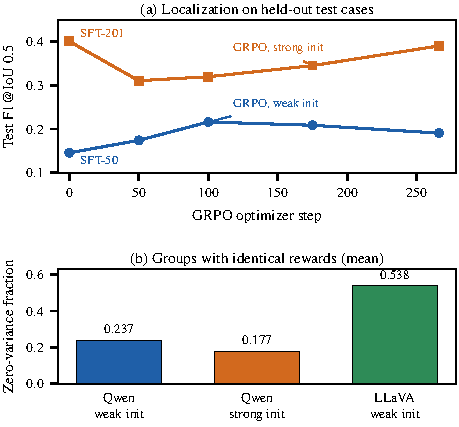
\includegraphics[width=0.94\columnwidth]{figures/fig_results.pdf}
\caption{(a) Test localization F1@0.5 during GRPO from a weak (SFT-50) and a strong (SFT-201) initialization. Step 0 is the SFT policy. (b) Mean fraction of GRPO groups whose four sampled rewards are identical; such groups produce zero advantage. }
\label{fig:results}
\end{figure}

\subsection{Why the Reward Signal Fades}
Fig.~\ref{fig:results}(b) shows the fraction of groups with identical rewards. With $G=4$, 23.7\% of Qwen's groups from the weak initialization and 17.7\% from the strong initialization have zero reward variance; for LLaVA the figure is 53.8\%. A zero-variance group contributes no reward-advantage gradient (the KL term may still contribute), and the reward is especially sparse because localization uses a hard IoU threshold: a box that misses by a few pixels receives the same zero as a box on the wrong hemisphere. The coarse diagnosis match further coarsens the signal.

Caption quality is not directly rewarded; its small change is therefore unsurprising, although shared parameters can change unrewarded outputs. The diagnosis reward is more revealing: during GRPO from SFT-201, the training diagnosis reward rises from 0.17 to 0.25, but test keyword Top-1 falls from 0.108 to 0.099. This is compatible with overfitting or reward--evaluation mismatch, but does not prove memorization. Although 93.7\% of test images have labels absent from the fine-tuning set, a pretrained model can still generate them; low exact-match accuracy is not mathematically forced by this split.

\subsection{Data-Side Ablations}
We also tested two data-side variants. The v2 dataset renders boxes as integers, adds 25\% auxiliary localization-only samples, and cleans final diagnoses; v3 reduces the auxiliary fraction to 10\%. Both improve validation localization (raw F1@0.5 0.482 and 0.465 vs.\ 0.375 for SFT-201) and reduce size-dependent box bias, yet test raw F1@0.5 falls to 0.356 and 0.345, and calibrated F1@0.5 is 0.392/0.395 vs.\ 0.407; the calibrated comparison CIs include zero. The same val-to-test pattern appears without RL, consistent with sampling variability or distribution differences across splits. Because several data changes and training steps differ together, these variants do not isolate a single causal factor.

\subsection{Diagnosis and the Clinical-History Prior}
Diagnosis is weak across the board: keyword Top-1 is 0.09--0.14 and Top-5 is 0.17--0.25. A text-only Qwen model, given the same format-guided prompt without the image, reaches Top-1 0.171 and Top-5 0.171, while the image-conditioned zero-shot model reaches 0.108/0.189. This is a separate matched, format-guided comparison, not the main-table zero-shot prompt. Its point estimates suggest a substantial history/pretraining prior, but without a paired CI or ablations of the adapted models they do not establish that images are generally unhelpful. We do not claim that the image is uninformative in principle, only that this reward and evaluation do not demonstrate an image-specific gain.

\section{Discussion}

\paragraph{Interpreting the initialization comparison.} The early-start run has a transient localization gain, whereas the final-SFT start has no detected test gain. The evidence answers RQ1--RQ2 only for these runs, not for all SFT initializations. Sparse rewards, low box diversity, calibration shifts, overfitting, and split variability are plausible explanations for RQ3; they were not independently ablated. In particular, absence of a significant difference does not establish saturation or rule out optimization problems.

\paragraph{Why diagnosis remains difficult.} String rewards may favor familiar labels, while a hand-built alias metric can reward broad entities without clinical specificity. Label novelty, pretraining knowledge, history priors, and evaluation mismatch are distinct factors. Retrieval, image/history ablations, and expert assessment could separate them.

\paragraph{Why GRPO.} It avoids a learned critic and directly consumes programmatic rewards. This suits our limited memory and terminal-score setting, though PPO with shared parameters or DPO using reward-derived pairs are alternatives. Increasing $G$, dynamic sampling, or a continuous IoU component may improve reward contrast, but are untested here. Zero-variance groups remove the reward gradient, not the KL gradient.

\paragraph{Lessons.} Compare RL against sufficiently trained SFT and a simple calibration baseline; validation loss alone did not select a strong localization checkpoint here. Monitor reward variance and prediction diversity. Fit calibration on validation, and report raw results separately. Finally, lock checkpoint and metric rules before a new evaluation: the nominal CIs here cannot correct retrospective selection.

\paragraph{Reproducibility.} Saved \texttt{args.json} and \texttt{logging.jsonl} record the actual runs; script defaults alone do not reproduce them. The accompanying \texttt{paper/REPRODUCE.md} gives dependencies, explicit SFT/GRPO overrides, prediction and evaluation commands, and the mapping from Table~\ref{tab:main} to saved results. The course submission should include these artifacts and the code/data preparation instructions.

\section{Limitations}
\label{sec:limitations}

The dataset is small (235 cases; 36 test cases) and only one split and training seed are used. Bootstrap CIs capture case sampling, not run-to-run variation. Test-informed checkpoint and metric changes introduce selection bias; a fresh test set is needed for confirmation. SFT-201 is a stronger final checkpoint, not a demonstrated optimum. NOVA is an evaluation-only benchmark; our training split departs from its intended protocol, and case separation cannot exclude public-source contamination in model pretraining. We test two backbones, LoRA, one RL algorithm, and one reward design, without a compute-matched continued-SFT control or reward/KL ablations. Automatic coordinates, unequal reward/evaluation preprocessing, and the custom AP proxy further limit interpretation. Captions and diagnosis are assessed by lexical proxies without radiologist review; the text-only check covers zero-shot models only.

\section{Conclusion}
We applied GRPO with deterministic localization and diagnosis rewards to structured brain MRI reporting. A retrospectively selected early-start checkpoint improves localization, but final GRPO does not show a reliable gain from either SFT initialization. Stronger SFT gives a larger point improvement than the early-start RL refinement; diagnosis and captioning show no reliable gains. Our contribution is an implemented RL formulation and an empirical analysis of its limits under small-data adaptation. The results motivate stronger supervised baselines, smoother rewards, and evaluation rules fixed before a new test, rather than a general claim that GRPO helps only under-trained models.

\bibliographystyle{IEEEtran}
\bibliography{refs}

\end{document}
